\documentclass[aps,
%prl,
twocolumn,
%showpacs,
superscriptaddress,groupedaddress]{revtex4}


\usepackage{amssymb}
\usepackage{amsmath}
\usepackage{float}
\usepackage{graphicx}
\usepackage{subfig}
\usepackage{mathrsfs}

\newcommand{\dmcomment}[1]{{\tt #1}}

\begin{document}

\title{Theory of the crossover from lasing to steady state superradiance}
\author{D. A. Tieri}
\affiliation{JILA, University of Colorado, Boulder}
\author{Minghui Xu}
\affiliation{JILA, University of Colorado, Boulder}
\author{J. Cooper}
\affiliation{JILA, University of Colorado, Boulder}
\author{D. Meiser}
\affiliation{Tech-X Corporation, 5621 Arapahoe Avenue,
             Boulder, Colorado 80303, USA.}
\author{M. J. Holland}
\affiliation{JILA, University of Colorado, Boulder}
\date{\today}

\begin{abstract}
  Lasing and steady state superradiance are two phenomena that may
  appear at first glance to be distinct, but in fact should be thought
  of as the two extreme limits of a continuous crossover. In a laser,
  the macroscopic field that stores the phase information is the
  intracavity light field, and the robustness of this phase is what
  leads to the coherence properties of the output light. In contrast,
  in steady-state superradiant systems, the coherence derives from the
  macroscopic collective dipole of a many-atom ensemble. In this
  paper, we develop a quantum theory that connects smoothly between
  these two extreme limits by showing that coherence can be
  simultaneously stored in both atoms and light. The properties of
  systems that lie in the superradiance, lasing and crossover
  parameter regions are contrasted and compared. We find that a
  crossover system can operate much farther above threshold than a
  typical laser system, and that this can allow the linewidth of the
  output light to be orders of magnitude smaller. Importantly for
  precision metrology applications, we find that in the superradiant
  limit, the linewidth is insensitive to fluctuations in the cavity
  length, while a system in the lasing limit produces light with the
  linewidth that is insensitive to fluctuations in the atomic
  transition energy.
\end{abstract}
\maketitle

\section{Introduction}
Since its first demonstration in 1960~\cite{maiman1960stimulated}, the
laser has had a profound impact on fundamental science research, and
has also become ubiquitous in other areas of society. Lasers are
integral to many areas of research and applications, ranging from
atomic and molecular physics research, atomic clocks, global
positioning system, nuclear fusion research, biology research,
medicine and consumer electronics.

Although many different types of lasers exist, with their key
parameters spanning many orders of magnitude, all lasers share the
same conceptual foundation.  A laser is a cavity quantum
electrodynamics (QED) system consisting of a gain medium inside of an
optical cavity.  We will oftentimes refer to the gain medium as
``atoms'' for brevity.  Lasers typically operate in the so called good
cavity regime of cavity QED where the linewidth of the cavity is much
narrower than the bandwidth of the gain medium.  The atoms generate a
coherent electromagnetic field in the cavity by means of stimulated
emission~\cite{PhysRev.112.1940}. Stimulated emission is a quantum
mechanical interference effect in which the presence of a large number
of photons in a certain mode of a light field increases the
probability that an atom will emit into that mode. The energy emitted
into the cavity field has to be replenished by some repumping
mechanism to achieve steady state operation. In a laser, the
macroscopic phase information that is associated with the coherence of
the generated radiation is stored in the light field.

Around the same time as the laser was first demonstrated, the effect
of superradiance was predicted~\cite{PhysRev.93.99}, and soon
thereafter, experimentally demonstrated.  Superradiance is a quantum
mechanical interference effect in which correlations between atoms
cause them to emit collectively.  Superradiance has most commonly been
considered as a pulsed phenomenon.  Atoms in an ensemble are prepared
in the excited state.  Spontaneous emission into one or a few spatial
modes is then enhanced via a quantum mechanical interference effect.
However, it has been known for some time that superradiance can also
occur in steady state~\cite{PhysRevLett.102.163601,
  PhysRevA.81.033847, PhysRevA.81.063827,PhysRevLett.89.253003} by
placing the atomic ensemble inside a cavity.  In contrast to lasers,
superradiance in steady-state requires a cavity with a much broader
linewidth than the atomic linewidth.  This regime is referred to as
the bad-cavity limit of cavity QED~\cite{PhysRevA.51.809,
  PhysRevLett.72.3815, ChenDeliciousLaser, HakenLaser,
  HakenLaserBook}.  The radiation produced in steady state
superradiance is also coherent.  However, in contrast to a laser, the
coherence is stored in the atomic medium.  Progress has recently been
made towards the experimental verification~\cite{ThompsonPaper} of
this proposal.

An important application of lasers is as a stable local oscillator for
optical atomic clocks and precision spectroscopy.  These lasers rely
on stabilization against reference cavities.  The most advanced such
lasers reach linewidths of $< 0.1 {\rm Hz}$ corresponding to quality
factors of $Q>10^{15}$~\cite{Cole:TenfoldReductionBrownianNoise}.  The
limiting factor in the way of further improvement of these local
oscillators are thermal vibrations of the dielectric coatings in the
cavity mirrors~\cite{PhysRevLett.101.260602}.  To overcome this
challenge, it has been proposed to use steady state superradiance based
on clock transitions to create an even more stable light
source~\cite{PhysRevLett.102.163601, ChenDeliciousLaser}.  However,
this proposal has challenges of its own.  First of all, in spite of the
enhancement that occurs due to superradiance, the produced intensity is
typically much lower than a conventional laser.  Second of all,
perturbations of atomic transition frequencies can potentially lead to
phase and frequency perturbations in the generated field.

Balancing the advantages and disadvantages of the two systems (lasers
and light sources based on steady state superradiance) leads to the
following question: Why not consider a cavity QED system in which
coherence is stored in both the light field and atoms on an equal
footing? The linewidth of such a system should be less sensitive to
thermal fluctuations of the cavity mirrors than a laser, and it should
be able to produce more output power than a device based on steady state
superradiance.

The focus of this paper is to consider the properties of such a hybrid
system, and to compare and contrast them to the properties of systems
based purely on lasing and systems based purely on steady state
superradiance.  To this end we develop a theoretical model that is
applicable throughout the entire crossover.  We analyze the model using
different levels of approximation: An exact method using SU(4)
operators, a semi-classical method based on {\it c}-Number Langevin
equations, a quantum phase diffusion model for the field amplitude, a
cumulant expansion of system expectation values, and a mean field model.
By comparing the results from these different models we clarify the
role played by quantum fluctuations and correlations\dmcomment{Dave: Can
you put in some specifics on what role these play}.

The rest of this paper is organized as follows.  In section~\ref{sec:Model}
we summarize the physical model upon which our analysis is based. In
\ref{sec:Methods} we discuss the different levels of approximation
and to what extent they are able to capture the various physical
signatures. In section \ref{sec:CrossoverCharacterization} we characterize the crossover. In section~\ref{sec:Results} we discuss our results on the
crossover.  Details of the computation are presented in appendices.


\section{Model}
\label{sec:Model}

We model our system as a collection of $N$ two-level atoms inside a
single mode optical cavity using the quantum Born-Markov master equation
to describe the open quantum system,
\begin{equation}
  \frac{d}{dt} \hat{\rho} =
  \frac{1}{i \hbar} \left[ \hat{H}, \hat{\rho} \right] +
  \hat{\mathcal{L}}\left[ \hat{\rho} \right],
\label{ME1Crossover}
\end{equation}
where,
\begin{equation}
\hat{H} = \frac{\hbar \omega_a}{2} \sum_{j=1}^{N} \hat{\sigma}^{z}_{j}
+ \hbar \omega_c \hat{a}^{\dagger}\hat{a}
+ \frac{\hbar \Omega}{2}  \sum_{j=1}^{N} \left(
    \hat{a}^{\dagger} \hat{\sigma}^{-}_{j} +
    \hat{\sigma}^{+}_{j} \hat{a} \right),
\end{equation}
and $\hat{\mathcal{L}}\left[ \hat{\rho} \right]$ denotes the
Liouvillian superoperator.

The Hamiltonian $\hat{H}$ describes the coherent evolution of the
coupled atom cavity system, where $\omega_{a}$ is the frequency
between the two levels of each of the atoms, and $\omega_c$ is the
frequency of the cavity mode. The Pauli spin matrices for the atoms
are $\hat{\sigma}_j^{+}$ ,$\hat{\sigma}_j^{-}$ and
$\hat{\sigma}_j^{z}$, and $\hat{a}$ is the annihilation operator of
the cavity mode. The atom-cavity coupling rate is $\Omega$. That we
take this to be the same for all items implies assumption of the
equivalence of the atom-cavity coupling at the positions of all of the
atoms. This could be achieved by strongly confining the ensemble in a
optical lattice potential at the antinodes of the cavity modefunction.

The incoherent evolution is described by the Liouvillian
$\hat{\mathcal{L}}\left[ \hat{\rho} \right]$,
\begin{eqnarray}
\hat{\mathcal{L}}\left[ \hat{\rho} \right] &=&
  -\frac{\kappa}{2}
  \left(
    \hat{a}^{\dagger} \hat{a} \hat{\rho}
    + \hat{\rho}  \hat{a}^{\dagger} \hat{a}
    - 2\hat{a} \hat{\rho} \hat{a}^{\dagger}
  \right)
\nonumber
\\
 &&-\frac{\gamma}{2} \sum_{j=1}^N
  \left(
   \hat{\sigma}_{j}^{+} \hat{\sigma}_{j}^{-} \hat{\rho}
   + \hat{\rho} \hat{\sigma}_{j}^{+} \hat{\sigma}_{j}^{-}
   - 2\hat{\sigma}_{j}^{-} \hat{\rho} \hat{\sigma}_{j}^{+}
  \right)
\nonumber
\\
 &&-\frac{w}{2} \sum_{j=1}^N
  \left(
   \hat{\sigma}_{j}^{-} \hat{\sigma}_{j}^{+} \hat{\rho}
   + \hat{\rho} \hat{\sigma}_{j}^{-} \hat{\sigma}_{j}^{+}
   - 2\hat{\sigma}_{j}^{+} \hat{\rho}  \hat{\sigma}_{j}^{-}
  \right),
\nonumber
\\
 &&+\frac{1}{2T_2} \sum_{j=1}^N
  \left(
   \hat{\sigma}_{j}^{z} \hat{\rho}  \hat{\sigma}_{j}^{z} - \hat{\rho}
  \right),
\end{eqnarray}
where $\hat{\rho}$ is the system's density matrix, $\kappa$ is the decay
rate of the cavity, $\gamma$ is the incoherent decay rate of the atoms,
$w$ is the incoherent repumping rate of the atoms, and $\frac{1}{T_2}$
is the inhomogeneous dephasing rate.

\section{Solution Methods}
\label{sec:Methods}

Introduction to be added providing the structure of increasing number
and increasing level of approximation....

Moving each of the subsections below to individual appendices....

Eq.~(\ref{ME1Crossover}) becomes increasingly complex with increasing
atom number $N$, since the associated Hilbert space scales as $2^N$.
Exact simulation methods, such as the quantum jump and quantum state
diffusion methods, are limited to $N\sim10$ with the cavity field basis
truncated to just a few photons.

The SU(4) solution method \cite{Hartmann:arXiv1201.1732}
\cite{Holland13} exploits an underlying permutation symmetry in
Eq.~(\ref{ME1Crossover}) to drastically reduce the number of basis
states needed to describe the problem, allowing systems with
$N\sim100$ to be treated. However to treat this many particles, the
cavity field basis must also be truncated to just a few photons. In
order to treat systems which have a larger number of photons, we
combine the SU(4) method with the quantum jump method
\cite{Dalibard92} \cite{Dum92} \cite{Knight98}. Even with the ability
to describe problems with larger photon number, $N\sim100$ is still
too few particles to describe many realistic experimental situations.

We therefore also describe the c-number Langevin equation method
\cite{Scully97, PhysRevA.47.1431}, which approximate the quantum
Langevin equations that are equivalent to Eq.~(\ref{ME1Crossover}).
These equations do not scale with $N$ in the same way, and therefore can
often be used to treat systems with large $N$ where an exact treatment
is not possible. Another method that does not scale with $N$ in the same
way is the mean field solutions of the quantum Langevin equations, along
with an analytic solution for the linewidth of the power spectrum, which
assumes Gaussian phase fluctuations and neglects amplitude fluctuations
\cite{HakenLaser, HakenLaserBook}. Finally, the cumulant expansion
method \cite{JPSJ.17.1100} does not scale exponentially with $N$, and
can therefore also be used to treat large systems. These methods are now
described in detail.


\subsection{SU(4) Numerical Simulation of the Master Equation}

Recently, we have developed a group-theoretic method for efficiently
simulating the quantum master equation~\cite{Holland13}. In brief, the
master equation, Eq.~(\ref{ME1Crossover}), can be expressed in terms of
generators of the SU(4) group, with the Hamiltonian part being,
\begin{eqnarray}
  &&\frac{1}{i\hbar}[H,\rho]=
  -2i \omega_a \Sigma_3\rho -i\omega_c [ \hat{a}^{\dagger}\hat{a}, \rho]
  \nonumber
  \\
  &&-i\Omega \left[a(\mathcal{M}_++\mathcal{N}_+)\rho+a^\dagger
    (\mathcal{M}_-+\mathcal{N}_-)\rho\right]\nonumber\\
  &&\quad{}+i\Omega\left[(\mathcal{U}_++\mathcal{V}_+)\rho a^\dagger
    +(\mathcal{U}_-+\mathcal{V}_-)\rho a\right]\,,
\end{eqnarray}
and dissipation parts being,
\begin{eqnarray}\label{liv}
 && \sum_{j=1}^N(
   2\sigma_j^-\rho\sigma_j^+-\sigma_j^+ \sigma_j^-\rho-
   \rho \sigma_j^+\sigma_j^-
  )/2=-\frac{N}{2}-
  \mathcal{Q}_3+\mathcal{Q}_{-}\,,\nonumber\\
 && \sum_{j=1}^N(
   2\sigma_j^+\rho\sigma_j^--\sigma_j^- \sigma_j^+\rho-
   \rho \sigma_j^-\sigma_j^+
  )/2=-\frac{N}{2}+
  \mathcal{Q}_3+\mathcal{Q}_{+}\,,\nonumber\\
 && \sum_{j=1}^N(\sigma_j^{(3)}\rho\sigma_j^{(3)}-\rho)=4\mathcal{M}_3-2
  \mathcal{Q}_3-2\Sigma_3-N\,,
  \label{ham}
\end{eqnarray}
where $\mathcal{Q}_{\pm}$, $\mathcal{M}_{\pm}$, $\mathcal{N}_{\pm}$,
$\mathcal{U}_{\pm}$, $\mathcal{V}_{\pm}$, $\mathcal{Q}_3$, $\mathcal{M}_3$,
and $\Sigma_3$ are superoperators~\cite{Holland13}.  As a result, we can
expand the density matrix in terms of the fully symmetrical multiplet
$P_{q,q_3,\sigma_3}$~\cite{Holland13} of the SU(4) group,
\begin{equation}\label{ex}
  \rho=\sum_{q,q_3,\sigma_3,m,n} C_{q,q_3,\sigma_3}^{m,n}
  P_{q,q_3,\sigma_3}\bigl|m\bigr>\bigl<n\bigr|\,,
\end{equation}
where $C_{q,q_3,\sigma_3}^{m,n}$ are complex coefficients, and
$|n\rangle$ is the photon Fock state. Note that the total number of
states in the fully symmetrical multiplet is $1/6 (N+1)(N+2)(N+3)$,
which reduces the exponential scaling of the problem to cubic in $N$.
This has enabled us to numerically investigate large
systems~\cite{Holland13}.

However, the number of basis in Eq.~(\ref{ex}) also grows as square of
the photon number.  This would impose great difficulties in numerical
simulations of the laser region due to the large number of photons.
Below, we present a method that unravels the master equation in the
Liouville space, which enables us to remove the photon basis in the
simulation. The essential idea behind the method is that we are able to
deduce the photon state by keeping track of the total number of quanta
$N_q$ in the system.

\dmcomment{The following discussion should be made more precise.
Discuss what "random" means.}
The quantum Monte Carlo method decomposes the density operator evolution
into a set of quantum trajectories where, between applications of random
jumps into random channels, the system evolves under an effective
Hamiltonian~\cite{Dalibard92,Dum92,Knight98}. While this has
conventionally been done with wavefunctions to reduce the numerical
complexity, here we apply the quantum trajectory algorithm in the
density matrix space in order to get rid of the photon basis in the
expansion of the density operator. To construct a single trajectory, we
first need to identify the jump operators. In our problem, there are
four decay channels: repumping, spontaneous emission, dephasing and
cavity decay. The corresponding jump operators $\mathcal{J}_i$ are
\begin{eqnarray}
\mathrm{Repumping:} \mathcal{J}_1\rho&=&
w\sum_{j=1}^N(\sigma_j^+\rho\sigma_j^-)=w\mathcal{Q}_{+}\rho\,,
\nonumber\\
\mathrm{Spontaneous\,\,emission:}  \mathcal{J}_2\rho&=&
\gamma\sum_{j=1}^N(\sigma_j^-\rho\sigma_j^+)=
\gamma \mathcal{Q}_{-}\rho\,,\nonumber\\
\mathrm{Dephasing:} \mathcal{J}_3\rho&=&
\frac{1}{2T_2}\sum_{j=1}^N(\sigma_j^{(3)}\rho\sigma_j^{(3)})
\nonumber\\
&=&\frac{1}{2T_2}(4\mathcal{M}_3-2  \mathcal{Q}_3-2\Sigma_3)\rho\,,
\nonumber\\
\mathrm{Cavity\,\,decay:}  \mathcal{J}_4\rho&=&\kappa a\rho a^{\dagger}\,.
\label{jumpo}
\end{eqnarray}
When a repumping quantum jump happens, $N_q$ is decreased by one. When a
spontaneous emission or a cavity-decay quantum jump happens, $N_q$ is
increased by one. The dephasing quantum jump also does not change the
total number of quanta. Therefore, during the evolution of a single
trajectory, one could calculate $N_q$ at every time step by tracking the
the numbers of jumps of the different types. With the knowledge of
$N_q$, the photon state can be easily deduced. It is shown in
Ref.~\cite{Holland13} that
\begin{equation}
\begin{split}
  \hat{J}_3P_{q,q_3,\sigma_3}^{(\mathrm{s})}&=
  (q_3+\sigma_3)P_{q,q_3,\sigma_3}^{(\mathrm{s})},\\
  P_{q,q_3,\sigma_3}^{(\mathrm{s})}\hat{J}_3&=
  (q_3-\sigma_3)P_{q,q_3,\sigma_3}^{(\mathrm{s})},
\end{split}
\end{equation}
where $\hat{J}_3=\sum_{j=1}^N\sigma_j^{(3)}/2$ is the collective spin
operator. Therefore, the atomic state for a particular fully symmetrical
atomic basis in terms of the number of excited atoms is
$|q_3+\sigma_3+N/2\rangle\langle q_3-\sigma_3+N/2|$. And thus the
corresponding photon state is
\begin{equation}
\bigl|m\bigr>\bigl<n\bigr|=
\bigl|N_q-(q_3+\sigma_3+N/2)\bigr>
\bigl<N_q-(q_3-\sigma_3+N/2)\bigr|.
\end{equation}
Therefore, by counting the quantum jumps, we have complete knowledge of
photon states for every single trajectory. This enables us to remove the
photon basis, which greatly improves the efficiency of the method.

\dmcomment{Does the efficiency improvement rely on starting out in
a photon number state? If so we should probably comment on that.}

The simulation of jump times and jump channels is completely analogous
to the wave-function Monte Carlo method. The effective evolution of the
system is governed by the master equation excluding the above jump
operators. As a result, under the effective evolution, the trace of the
density operator is no longer conserved, but decreases as a function of
time.  This is analogous to the decay of the norm of the wavefunction in
the wave function Monte Carlo method. A jump occurs when the trace of
the density operator is less than a random number uniformly distributed
in the interval $[0,1]$. When a decay occurs we stochastically determine
the channel $i$ into which the system decays according to the
probability distribution,
\begin{equation}
\mathcal{P}_i^{\mathrm{jump}}=\frac{\mathrm{Tr}[\mathcal{J}_i\rho]}{\sum_{k=1}^4
\mathrm{Tr}[\mathcal{J}_k\rho]}.
\end{equation}

Finally, in order to get the density operator at each time step, an
ensemble average of many quantum trajectories is required. Then, various
observables can be calculated according to Ref.~\cite{Holland13}. It is
also worth noting that if one is only interested in the steady state
density operator, a time average in the steady state can be applied
instead of the ensemble average.


\subsection{Langevin Theory}

The Langevin equations equivalent to Eq.~(\ref{ME1Crossover}) are given
by,
\begin{equation}
\frac{d}{dt} \hat{a}= -\frac{1}{2} (\kappa +2i\omega_c) \hat{a}
-\frac{i N \Omega}{2} \hat{S}^{-}
+\hat{F}^{a},
\label{La}
\end{equation}
\begin{equation}
\frac{d}{dt} \hat{S}^{-} =
-\frac{1}{2} \left(\Gamma +2 i \omega_a \right)  \hat{S}^{-}
+\frac{i \Omega}{2} \hat{a} \hat{S}^{z}
+\hat{F}^{-},
\label{Lsm}
\end{equation}
\begin{equation}
\frac{d}{dt} \hat{S}^{z} =
-(w+\gamma)\left( \hat{S}^{z} - d_0\right)
+i\Omega \left( \hat{a}^{\dagger}\hat{S}^{-} -
\hat{a}\hat{S}^{+} \right)
+\hat{F}^{z},
\label{Lsz}
\end{equation}
where $\delta=\omega_{a}-\omega_{c}$, where we have defined the collective
operators,
\begin{equation}
\hat{S}^{(+,-,z)}=\frac{1}{N}\sum_{k=1}^N \hat{\sigma}_k^{(+,-,z)},
\nonumber
\end{equation}
where $\Gamma \equiv w+\gamma+\frac{2}{T_2}$, and where $d_0 =
\frac{w-\gamma}{w+\gamma}$. The noise terms $\hat F^\mu$ are correlated
according to,
\begin{equation}
\left< \hat{F}^{\mu}(t) \hat{F}^{\nu}(t^{\prime})\right> =
2 D^{\mu \nu} \delta(t-t^{\prime}),
\end{equation}
where the $D^{\mu \nu} $ are calculated using the Einstein relations
\cite{meystre2007elements},
\begin{eqnarray}
&& 2D^{a a^{\dagger}}= \kappa \nonumber \\
&& 2D^{+-}= \frac{1}{N}
\left(
  w + \frac{1}{T_2} \left(1 + \left< \hat{S}^{z} \right> \right)
\right) \nonumber \\
&& 2D^{-+}= \frac{1}{N}
\left(
  \gamma + \frac{1}{T_2} \left(1- \left< \hat{S}^{z} \right> \right)
\right) \nonumber \\
&& 2D^{+z}= -\frac{2w}{N} \left< \hat{S}^{+} \right>
\hspace{0.83in} 2D^{z+}= \frac{2\gamma}{N} \left< \hat{S}^{+} \right>
\nonumber \\
&& 2D^{-z}= \frac{2\gamma}{N} \left< \hat{S}^{-} \right>
\hspace{0.86in} 2D^{z-}= -\frac{2w}{N} \left< \hat{S}^{-} \right>
\nonumber \\
&& 2D^{zz}= \frac{2\gamma}{N}
\left(1+ \left< \hat{S}^{z} \right> \right) +
\frac{2w}{N}\left(1- \left< \hat{S}^{z} \right> \right).
\label{OpNoise1}
\end{eqnarray}


\subsubsection{C-number Langevin equations for numerical simulations}

Eqns.~(\ref{La}~--~\ref{Lsz}) are operator equations, and are therefore
difficult to simulate on a computer. We therefore derive c-number
Langevin equations that correspond to the operator equations.  The
c-number equations are constructed in such a way that they reproduce the
correct first and second moments of certain operators.

Since operators do not necessarily commute, and c-numbers do, care must
be taken in making this correspondence. We define,
\begin{equation}
\frac{d}{dt} a= -\frac{1}{2}  (\kappa +2i\omega_c) a
-\frac{i N \Omega}{2} S^{-}
+F^{a},
\label{Lac}
\end{equation}
\begin{equation}
\frac{d}{dt} S^{-} = -\frac{1}{2}  \left(\Gamma +2 i \omega_a \right)  S^{-}
+\frac{i \Omega}{2} a S^{z}
+F^{-},
\end{equation}
\begin{equation}
\frac{d}{dt} S^{z} = -(w+\gamma)\left( S^{z} - d_0\right)
+i\Omega \left( a^{\dagger}S^{-} - a S^{+} \right)
\label{Lszc}
+F^{z},
\end{equation}
where the omission of the hats over the variables signifies that they
are c-numbers. The noise terms are correlated according to,
\begin{equation}
\left< F^{\mu}(t) F^{\nu}(t^{\prime})\right> =
2 \mathscr{D}^{\mu \nu} \delta(t-t^{\prime}),
\end{equation}
where the elements of $\mathscr{D}^{\mu \nu}$ depend on the precise
operator ordering that is chosen.

\dmcomment{Need to clean up the following paragraph}
The elements of $\mathscr{D}^{\mu \nu}$ can be determined by using
Eqns.~(\ref{Lac}~--~\ref{Lszc}) to derive equations of motion for the
c-number second order moments, since those equations of motion contain
the elements of $\mathscr{D}^{\mu \nu}$ (i.e. $\mathscr{D}^{\mu \nu} =
\left<A^{\mu}F^{\nu}\right>=\left<F^{\mu}A^{\nu}\right>$ where $A^{\mu}$
is a system variable). Equations of motion for the operator second order
moments using Eqns.~(\ref{La}~--~\ref{Lsz}) must then also be derived. A
correspondence is then made by choosing an ordering for the operators,
and enforcing that the c-number second order moment equations are equal
to the operator second order moment equations for that ordering.

\dmcomment{"c-numbers commute" is a bit repetitive}
To illustrate the procedure, we note that since c-numbers commute,
$\left<S^{+}S^{-} \right> = \left<S^{-}S^{+} \right>$, and they also
have the same equations of motion,
\begin{eqnarray}
\frac{d}{dt} \left<S^{+}S^{-} \right>  \hspace{-0.03in} &=&
\hspace{-0.03in}  - \Gamma  \left< S^{+} S^{-} \right>
-\frac{i \Omega}{2} \left< a^{\dagger} S^{z} S^{-} \right>
\nonumber
\\
 && +\frac{i \Omega}{2} \left< a S^{+} S^{z} \right> + 2 \mathscr{D}^{+-}.
 \label{c2om1}
\end{eqnarray}

Since operators don't commute, there are several options for operator
second order moment equations that could correspond to
Eq.~(\ref{c2om1}). For instance,
\begin{eqnarray}
\frac{d}{dt} \left<\hat{S}^{+}\hat{S}^{-} \right>  \hspace{-0.03in} &=&
\hspace{-0.03in}  - \Gamma  \left< \hat{S}^{+} \hat{S}^{-} \right>
-\frac{i \Omega}{2} \left< \hat{a}^{\dagger} \hat{S}^{z} \hat{S}^{-} \right>
\nonumber
\\
 &&+\frac{i \Omega}{2}  \left< \hat{a} \hat{S}^{+} \hat{S}^{z} \right>  +
 2 D^{+-},
\end{eqnarray}
\begin{eqnarray}
\frac{d}{dt} \left<\hat{S}^{-}\hat{S}^{+} \right>  \hspace{-0.03in} &=&
\hspace{-0.03in}  - \Gamma  \left< \hat{S}^{-} \hat{S}^{+} \right>
-\frac{i \Omega}{2} \left< \hat{a}^{\dagger} \hat{S}^{z} \hat{S}^{-} \right>
\nonumber
\\
 &&+\frac{i \Omega}{2}  \left< \hat{a} \hat{S}^{+} \hat{S}^{z} \right>  +
 2 D^{-+},
\end{eqnarray}
\begin{eqnarray}
\frac{d}{dt} \left<\hat{S}^{+}\hat{S}^{-} \right>_s  \hspace{-0.03in} &=&
\hspace{-0.03in}  - \Gamma  \left< \hat{S}^{+} \hat{S}^{-} \right>_s
-\frac{i \Omega}{2} \left< \hat{a}^{\dagger} \hat{S}^{z} \hat{S}^{-} \right> _s
\nonumber
\\
 &&+\frac{i \Omega}{2}  \left< \hat{a} \hat{S}^{+} \hat{S}^{z} \right>_s +
 D^{+-} +D^{-+},
 \nonumber
\\
\end{eqnarray}
are all equally valid, where the symmetric expectation value of two
operators $\hat{A}$ and $\hat{B}$ is given by $\left< \hat{A} \hat{B}
\right>_s=\frac{1}{2} \left( \left< \hat{A} \hat{B} \right> + \left<
\hat{B} \hat{A} \right> \right)$. Therefore, depending on the ordering
chosen, $2 \mathscr{D}^{+-}$ can either be equal to $2 D^{+-}$,  $2
D^{-+}$ , or $D^{+-}+D^{-+}$. All orderings are equally valid, but one
must be chosen, and consistently used. The difference lies in the
inability of the semiclassical theory to completely describe the full
predictions of quantum mechanics.
\dmcomment{This discussion needs to be tightened up a bit}

With this in mind, we make our correspondence, by first changing
variables to,
\begin{equation}
\hspace{-0.5in} \hat{q} =
\frac{1}{2} \left( \hat{a}^{\dagger} + \hat{a} \right)
\hspace{0.5in} \hat{p} =
\frac{1}{2i} \left( \hat{a}^{\dagger} - \hat{a} \right)
\end{equation}
\begin{equation}
\hat{S}^x =
\frac{1}{2} \left( \hat{S}^{+} + \hat{S}^{-} \right)
\hspace{0.2in} \hat{S}^y =
\frac{1}{2i} \left( \hat{S}^{+} - \hat{S}^{-} \right).
\end{equation}
This allows us to deal with real quantities only, and therefore by this
construction, the c-number equations will have $a^{\dagger}$ complex
conjugate to $a$, and $S^+$  complex conjugate to $S^-$.

We choose to match the c-number second order moments to the
symmetrically ordered quantum second order moments. This ordering is
chosen since, by construction, this correspondence will always give
$2\mathscr{D}^{\mu \nu}=D^{\mu \nu}+D^{\nu \mu}$, i.e. there are never
any left over commutator pieces in $\mathscr{D}^{\mu \nu}$. The c-number
equations with this symmetric noise are given by,
\begin{equation}
\frac{d}{dt} q= -\kappa q - 2 \omega_c p - N \Omega S^{y} + F^{q},
\label{cq1}
\end{equation}
\begin{equation}
\frac{d}{dt} p= -\kappa p + 2 \omega_c q + N \Omega S^{x} + F^{p},
\end{equation}
\begin{equation}
\frac{d}{dt} S^{x} =
-\Gamma S^{x}  - 2 \omega_a S^{y} + \Omega p S^{z} + F^{x},
\end{equation}
\begin{equation}
\frac{d}{dt} S^{y} =
-\Gamma S^{y}  + 2 \omega_a S^{x} - \Omega q S^{z} + F^{y},
\end{equation}
\begin{equation}
\frac{d}{dt} S^{z} = -(w+\gamma)\left( S^{z} - d_0\right)
+2 \Omega \left( q S^{y} - p S^{x} \right)
+F^{z},
\end{equation}
with,
\begin{eqnarray}
&& 2\mathscr{D}^{q q}=
\frac{\kappa}{4} \hspace{0.7in} 2\mathscr{D}^{p p}=
\frac{\kappa}{4} \nonumber \\
&& 2\mathscr{D}^{xx}=
\frac{\Gamma}{4N} \hspace{0.57in} 2\mathscr{D}^{yy}=
\frac{\Gamma}{4N} \nonumber \\
&& 2\mathscr{D}^{xz}=
2\mathscr{D}^{zx}=
\frac{-w+\gamma}{N} \left< \hat{S}^{x} \right>  \nonumber \\
&& 2\mathscr{D}^{yz}=
2\mathscr{D}^{zy}=
\frac{-w+\gamma}{N} \left< \hat{S}^{y} \right>  \nonumber \\
&& 2\mathscr{D}^{zz}=
\frac{2}{N}\left((w+\gamma) + (-w+\gamma)  \left< \hat{S}^{z} \right> \right).
\label{cNoise1}
\end{eqnarray}
Symmetric ordering also gives the added benefit that $\mathscr{D}^{\mu
\nu}$ is by construction symmetric, which allows us to use a simple
algorithm to find the noises $F^\mu$ for a computer simulation that will
reproduce $\mathscr{D}^{\mu \nu}$.  The noises are found by finding the
unitary transformation that diagonalizes $\mathscr{D}^{\mu \nu}$, and
then applying the inverse transformation to the product of the square
root of each of its eigenvalues with an independent Wiener process. This
gives the correct linear combination of independent Wiener processes
that reproduces $\mathscr{D}^{\mu \nu}$.
Eqns.~(\ref{cq1}~--~\ref{cNoise1}) are equivalent to a Fokker-Planck
equation for the Wigner quasi-probability distribution.


\subsubsection{Mean Field Langevin}

Much physical insight into our system can be gained by considering
analytical expressions derived with varying orders of quantum
fluctuations. Since our system is composed of a large number of
constituent parts, the overall quantum fluctuations are expected to be
small. To this end, we first look at Eqns.~(\ref{La}~--~\ref{Lsz}) in
the limit that all quantum fluctuations are neglected by taking their
expectation values. In an interaction picture that rotates with the
frequency of the coupled atom cavity system $\omega$, these equations
become,
\begin{equation}
\frac{d}{dt} a_0= -\frac{1}{2} (\kappa +2i(\omega_c-\omega)) a_0
-\frac{i N \Omega}{2} S_0^{-},
\label{La0}
\end{equation}
\begin{equation}
\frac{d}{dt} S_0^{-} =
-\frac{1}{2} \left(\Gamma +2 i (\omega_a-\omega) \right)  S_0^{-}
+\frac{i \Omega}{2} \hat{a} S_0^{z},
\end{equation}
\begin{equation}
\frac{d}{dt} S_0^{z} = -(w+\gamma)\left( S_0^{z} - d_0\right)
+i\Omega \left( a_0^{\dagger} S_0^{-} - a_0 S_0^{+} \right).
\label{Lsz0}
\end{equation}
In steady state, Eqns.~(\ref{La0}~--~\ref{Lsz0}) yield that either
$a_0=0$, or,
\begin{equation}
S_0^{z}=
\frac{(\kappa+2i(\omega_c-\omega))(\Gamma+2i(\omega_a-\omega))}{N\Omega^2}.
\label{Sz01}
\end{equation}
Since $S_0^{z}$ must be real, we find
\begin{equation}
\omega = \frac{\kappa \omega_a + \Gamma \omega_c}{\kappa+\Gamma}.
\label{atomcavityfrequencycenter1}
\end{equation}
It is assumed that $\delta = \omega_a-\omega_c$ is small, so that terms
proportional to $\delta^2$ can be neglected. Then Eq.~\ref{Sz01} becomes,
\begin{equation}
S_0^{z}=\frac{1}{\mathcal{C}},
\end{equation}
where $\mathcal{C}\equiv \frac{N \Omega^2}{\kappa \Gamma}$ is the many-atom cooperativity. We also find,
\begin{equation}
|a_0|^2=\frac{N(w+\gamma)}{2 \kappa} (d_0 - \frac{1}{\mathcal{C}}).
\label{a0sqSS}
\end{equation}
Eq.~(\ref{a0sqSS}) is a quadratic function of $w$, and therefore has a maximum value. By setting the derivative of Eq.~(\ref{a0sqSS}) with respect to w equal to zero, the optimum value of $w$ which gives maximum $|a_0|^2$ can be found. It is given by,
\begin{equation}
w_{\mathrm{opt}} = \frac{N \Omega^2}{2\kappa} - \gamma - \frac{1}{T_2}.
\label{wopt}
\end{equation}
In the limit $\frac{N\Omega^2}{2 \kappa} >> \gamma, \frac{1}{T_2}$, then,
\begin{equation}
(|a_0|^2)_{\mathrm{opt}}= \frac{N^2 \Omega^2}{8\kappa^2}.
\label{adaopt}
\end{equation}
The first and second threshold are defined to be the values of w at which Eq.~(\ref{a0sqSS}) equals zero. It is assumed that the first threshold occurs at $w_1 \ll w_{opt}$. In this limit, Eq.~(\ref{a0sqSS}) set equal to zero yields,
\begin{equation}
w_1 = \gamma.
\label{FirstThreshold}
\end{equation} 
Eq.~(\ref{FirstThreshold}) tells us that the first threshold occurs when the repumping becomes greater than the natural linewidth of the atoms, when coherence can start to become established.
The second threshold occurs at $w_2 \sim w_{opt}$. In this limit, Eq.~(\ref{a0sqSS}) set equal to zero yields,
\begin{equation}
w_2 =  \frac{N \Omega^2}{\kappa}
\end{equation} 
At this point, $S_0^{z}$ is very close to unity, and the repumping destroys the coherence in the system.
\subsubsection{Phase Diffusion Linewidth}

\dmcomment{A bit of a rough transition here; could use some context}
The linewidth due to the phase fluctuations of $\hat{a}$ is now derived from the quantum Langevin equations, Eqns.~(\ref{La}~--~\ref{Lsz}) .
Following closely to the derivation done in \cite{HakenLaser,
HakenLaserBook}, Eq.~(\ref{La}) is differentiated, and substituted into
it Eqns.~(\ref{La}~--~\ref{Lsm}) and the integral of Eq.~(\ref{Lsz}), to
arrive at an equation for $\hat{a}$ alone,
\begin{equation}
\ddot{\hat{a}} =
-\frac{1}{2} (\kappa+\Gamma)  \dot{\hat{a}} -
\frac{\kappa \Gamma}{4}\hat{a}  +
\frac{N \Omega^2 }{4} \hat{a} \hat{S}^z +\hat{F},
\label{addeq}
\end{equation}
where
\begin{eqnarray}
\hat{S}^z &=&
\int_0^t dt^{\prime} e^{-(w+\gamma)(t-t^{\prime})}
\bigg( (w+\gamma) + \hat{F}^z
\nonumber
\\
&&-\frac{2}{N} \left( \frac{d}{dt} (\hat{a}^{\dagger} \hat{a}) +
\kappa \hat{a}^{\dagger} \hat{a} -\hat{a}^{\dagger} \hat{F}^a -
\hat{F}^{a^{\dagger}} \hat{a} \right) \bigg),
\end{eqnarray}
and,
\begin{equation}
\hat{F} = \frac{\Gamma}{2} \hat{F}^a-
\frac{i N \Omega}{2} \hat{F}^-+\dot{\hat{F}}^a.
\end{equation}
The annihilation operator $\hat{a}$ is decomposed according to,
\begin{equation}
\hat{a}= (a_0 + \hat{\rho}) e^{i\hat{\phi}}.
\label{adecomp}
\end{equation}
Above threshold, amplitude fluctuations are expected to be small, so that
\begin{equation}
\left< \hat{a}^{\dagger}(t) \hat{a}(0) \right> =
a_0^2 \left< e^{i(\hat{\phi}(t) - \hat{\phi}(0))} \right>.
\end{equation}

After substituting Eq.~(\ref{adecomp}) into Eq.~(\ref{addeq}), we take
the imaginary part to first order in products of operators, and find,
\begin{equation}
\ddot{\hat{\phi}} =
-\frac{1}{2}(\kappa+\Gamma) \dot{\hat{\phi}} +
\frac{1}{a_0} \text{Im} [\hat{F}],
\label{phieq1}
\end{equation}
where a factor of $e^{-i\phi}$ has been absorbed into $\hat{F}$.
Eq.~(\ref{phieq1}) is then integrateed, assuming that $(\kappa+\Gamma)$
is large, to arrive at,
\begin{equation}
\hat{\phi}(t) - \hat{\phi}(0) =
\frac{2}{a_0 (\kappa+\Gamma)}
\int_0^t dt^{\prime} \text{Im}
\left[ \frac{\Gamma}{2} \hat{F}^a-\frac{i N \Omega}{2} \hat{F}^-\right].
\label{phieq2}
\end{equation}
Since $ \hat{F}^a$ and $\hat{F}^-$ are Gaussian, we can use
\begin{equation}
\left< e^{i(\hat{\phi}(t) - \hat{\phi}(0))} \right> =
e^{-\frac{1}{2}\left< ( \hat{\phi}(t) - \hat{\phi}(0) )^2 \right>}.
\end{equation}
Therefore, we use Eq.~(\ref{phieq2}), along with Eqns.~(\ref{OpNoise1})
to find,
\begin{equation}
\left<(\hat{\phi}(t) - \hat{\phi}(0))^2 \right> =
\left(\frac{(C+1)}{2(Cd_0-1)} \frac{\Gamma}{(w+\gamma)}
\frac{\Omega^2 \kappa}{(\kappa+\Gamma)^2}\right) t,
\end{equation}
so that the linewidth $\Delta \nu$ given by,
\begin{equation}
\Delta \nu =
\frac{(C+1)}{2(Cd_0-1)} \frac{\Gamma}{(w+\gamma)}
\frac{\Omega^2 \kappa}{(\kappa+\Gamma)^2}.
\label{LWHaken}
\end{equation}


\subsection{Second Order Cumulant Theory}

The cumulant theory is derived by using Eq.~(\ref{ME1Crossover}) to find
equations for expectation values of system observables, which are
truncated to second order in a cumulant expansion, resulting in the
closed set of equations,
\begin{equation}
\frac{d}{dt} \left<\hat{\sigma}_{1}^{z}\right> =
-(w+\gamma)\left( \left<\hat{\sigma}_{1}^{z}\right> - d_0\right)
+i\Omega \left( \left<\hat{a}^{\dagger}\hat{\sigma}_{1}^{-}\right> -
\left<\hat{a}\hat{\sigma}_{1}^{+}\right> \right)
\label{szCE1}
\end{equation}
\begin{eqnarray}
\frac{d}{dt} \left<\hat{a}^{\dagger}\hat{\sigma}_{1}^{-}\right>
&=& -\frac{1}{2}(\Gamma+\kappa-2 i \delta)
\left<\hat{a}^{\dagger}\hat{\sigma}_{1}^{-}\right>
+\frac{i \Omega}{2} \bigg\{
\left<\hat{a}^{\dagger}\hat{a}\right> \left<\hat{\sigma}_{1}^{z}\right>
\nonumber
\\
&&
+ \frac{1}{2} \left(  \left<\hat{\sigma}_{1}^{z}\right> + 1 \right)
+ (N-1) \left<\hat{\sigma}_{1}^{+}\hat{\sigma}_{2}^{-}\right>
\bigg\}
\end{eqnarray}
\begin{equation}
\frac{d}{dt} \left<\hat{\sigma}_{1}^{+}\hat{\sigma}_{2}^{-}\right> =
-\Gamma \left<\hat{\sigma}_{1}^{+}\hat{\sigma}_{2}^{-}\right> +
\frac{\Omega}{2i} \left< \hat{\sigma}_{1}^{z} \right>
\left( \left<\hat{a}^{\dagger}\hat{\sigma}_{1}^{-}\right> -
\left<\hat{a}\hat{\sigma}_{1}^{+}\right> \right)
\end{equation}
\begin{equation}
\frac{d}{dt} \left<\hat{a}^{\dagger}\hat{a}\right> =
-\kappa \left<\hat{a}^{\dagger}\hat{a}\right>
+\frac{N \Omega}{2i}
\left( \left<\hat{a}^{\dagger}\hat{\sigma}_{1}^{-}\right> -
\left<\hat{a}\hat{\sigma}_{1}^{+}\right> \right).
\label{adaCE1}
\end{equation}
\dmcomment{Steady state of cumulant eqns provide initial conditions;
quantum regression theorem provides equations of motion for two-time
correlation functions}  This second order cumulant expansion, along with
the quantum regression theorem, can be used to find a closed set of
equations for two-time expectation values,
\begin{equation}
\frac{d}{d\tau}
\left[ \begin{array}{c}
\left<\hat{a}^{\dagger}(\tau)\hat{a}(0)\right> \\
\left<\hat{\sigma}_{1}^{+}(\tau)\hat{a}(0)\right>  \\
\end{array} \right]
=
\left[ \begin{array}{cc}
-\frac{\kappa}{2} +i \delta & \frac{iN\Omega}{2}  \\
-\frac{i\Omega\left<\hat{\sigma}_{1}^{z}\right>}{2}& -\frac{\Gamma}{2}  \\
\end{array} \right]
\left[ \begin{array}{c}
\left<\hat{a}^{\dagger}(\tau)\hat{a}(0)\right> \\
\left<\hat{\sigma}_{1}^{+}(\tau)\hat{a}(0)\right>  \\
\end{array} \right].
\label{TwoTimeCE1}
\end{equation}
These equations are written in a frame rotating at the atomic frequency.
They are important, since the Fourier transform of
$\left<\hat{a}^{\dagger}(\tau)\hat{a}(0)\right>$ is the spectrum of the
light inside our cavity QED system.  \dmcomment{Discussion of importance
of this equation should be moved up}


\dmcomment{Laplace transform is one way to solve the equations} By using
Laplace transform methods, it is found that the solution of the
$\left<\hat{a}^{\dagger}(\tau)\hat{a}(0)\right>$ equation, of
Eq.~(\ref{TwoTimeCE1}) is dominated by a single exponential with decay
constant,
\begin{equation}
\Delta \nu = \frac{1}{2}(\kappa+\Gamma-2i\delta) -
\frac{1}{2} \sqrt{(-\kappa+\Gamma+2i\delta)^2 +
4N\Omega^2 \left<\hat{\sigma}_{1}^{z}\right>},
\label{LW1}
\end{equation}
and hence the spectrum is a Lorentzian with linewidth given by
Eq.~(\ref{LW1}).

\begin{figure*}
\begin{center}
	\rotatebox{90}{\hspace{4mm} \textbf{Superradiance}}
	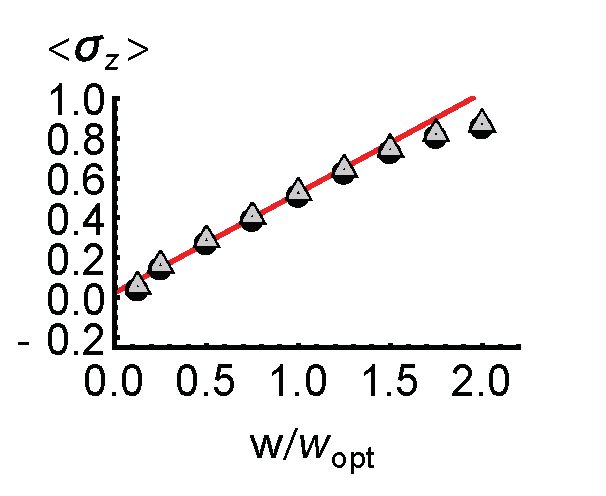
\includegraphics[scale =0.38] {N40SuperradianceSZ.eps}
	\hspace{-5.0mm} 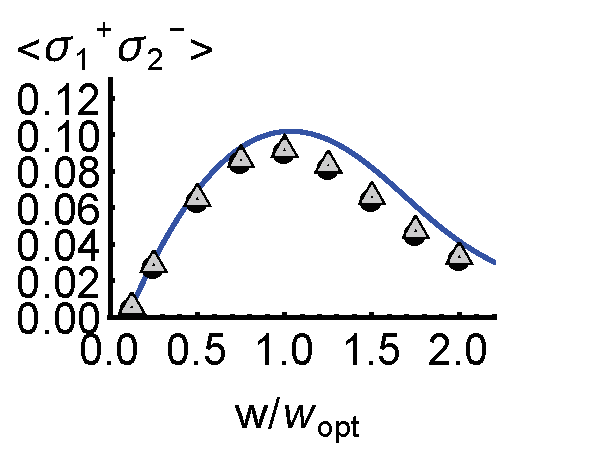
\includegraphics[scale =0.38] {N40SuperradianceSPSM.eps}
	\hspace{-5.0mm} 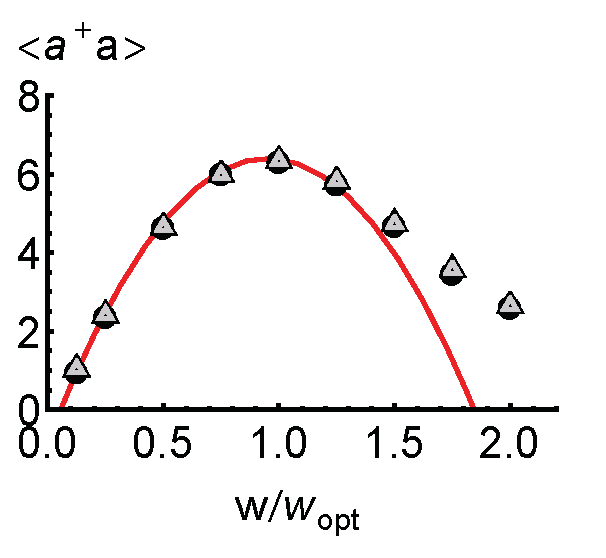
\includegraphics[scale =0.38] {N40Superradianceada.eps}
	\hspace{-5.0mm} 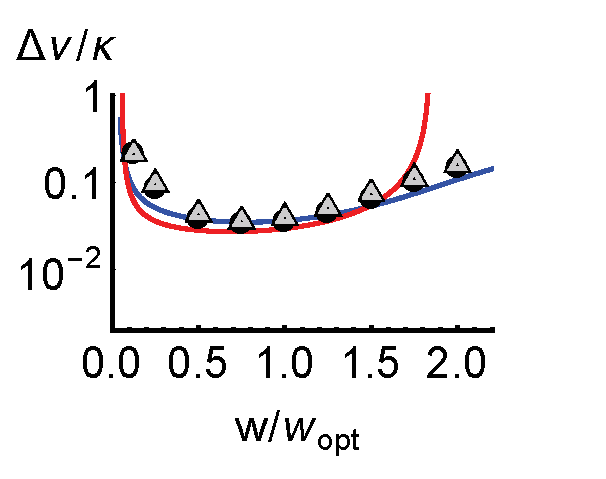
\includegraphics[scale =0.38] {N40SuperradianceLW.eps}
	\hspace{-5.0mm} 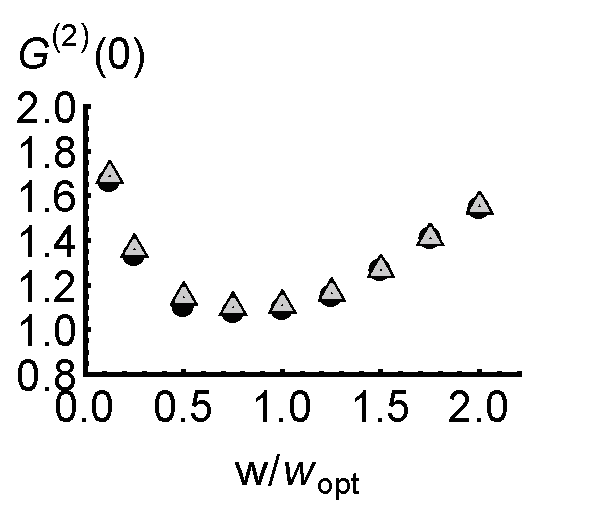
\includegraphics[scale =0.38] {N40SuperradianceG2.eps}\\ \vspace{0mm}
	\rotatebox{90}{ \hspace{7mm} \textbf{Crossover}}
	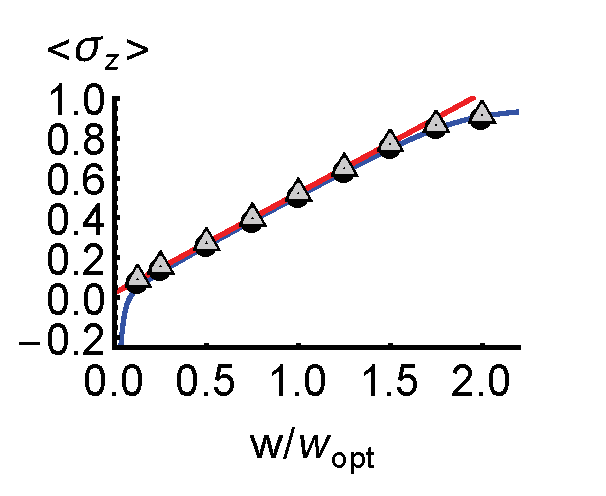
\includegraphics[scale =0.38] {N40CrossoverSZ.eps}
	\hspace{-5.0mm} 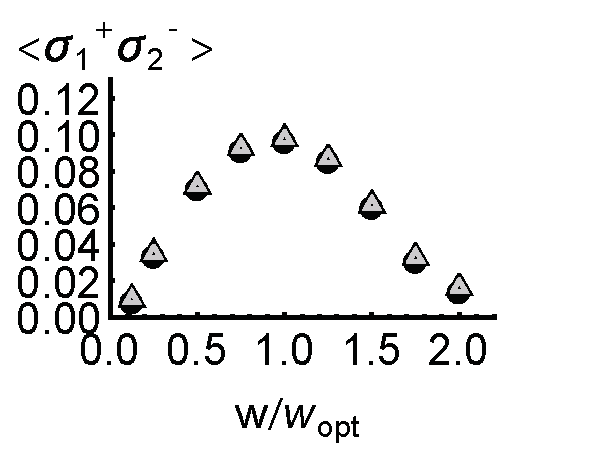
\includegraphics[scale =0.38] {N40CrossoverSPSM.eps}
	\hspace{-5.0mm} 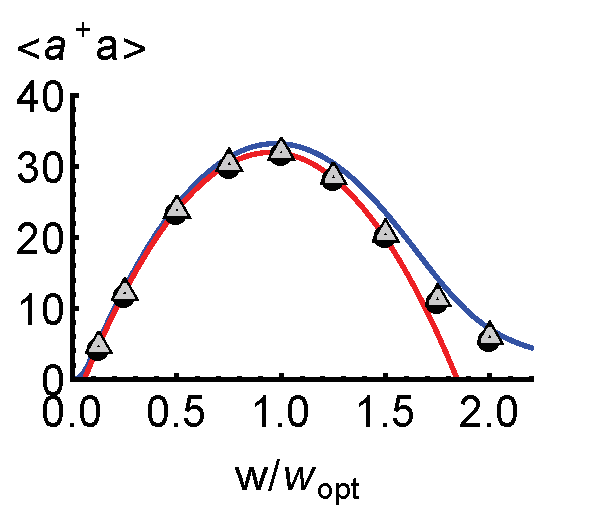
\includegraphics[scale =0.38] {N40Crossoverada.eps}
	\hspace{-5.0mm} 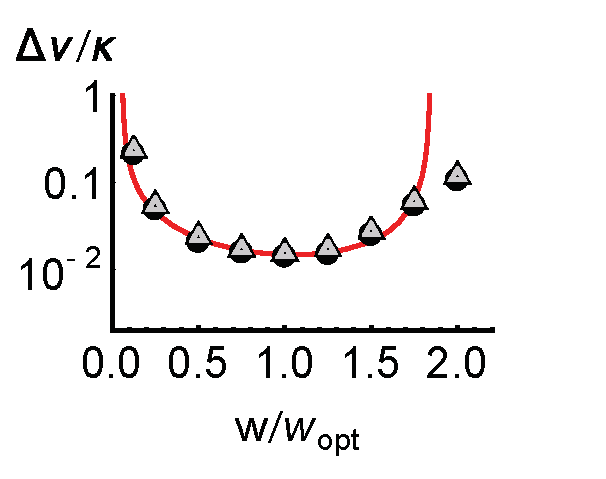
\includegraphics[scale =0.38] {N40CrossoverLW.eps}
	\hspace{-5.0mm} 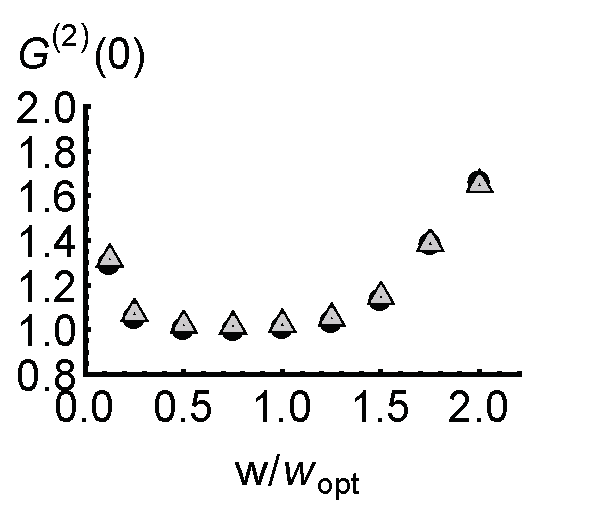
\includegraphics[scale =0.38] {N40CrossoverG2.eps}\\ \vspace{0mm}
	\rotatebox{90}{ \hspace{10mm} \textbf{Lasing}}
	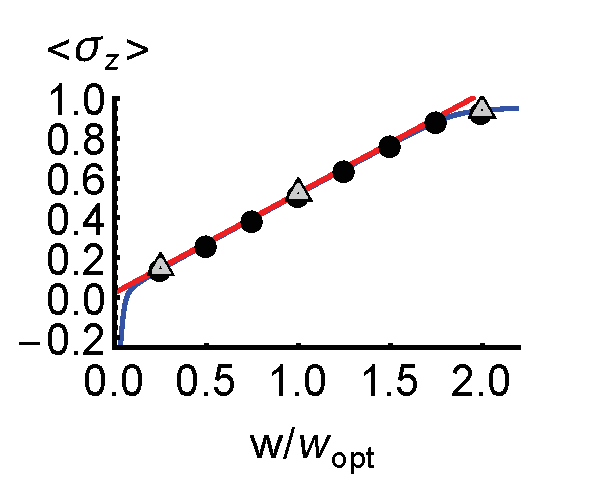
\includegraphics[scale =0.38] {N40LaserSZ.eps}
	\hspace{-5.0mm} 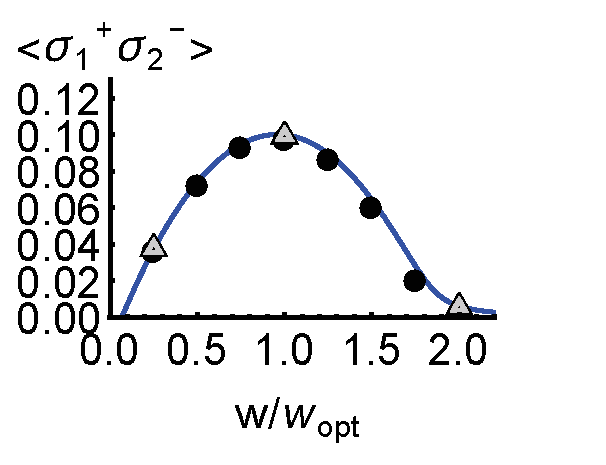
\includegraphics[scale =0.38] {N40LaserSPSM.eps}
	\hspace{-5.0mm} 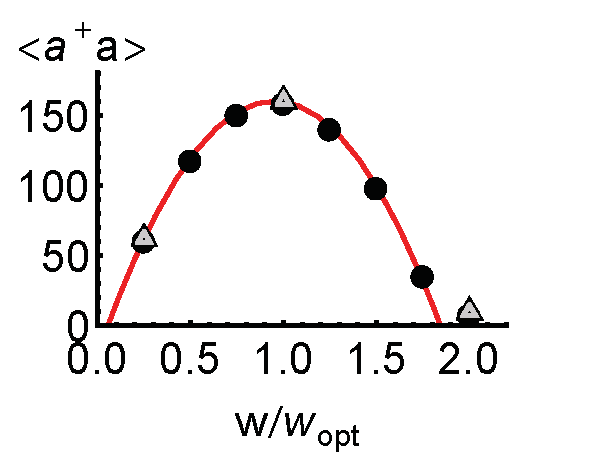
\includegraphics[scale =0.38] {N40Laserada.eps}
	\hspace{-5.0mm} 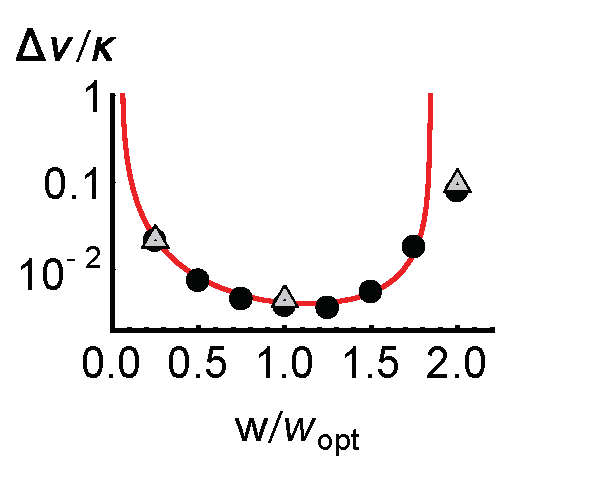
\includegraphics[scale =0.38] {N40LaserLW.eps}
	\hspace{-5.0mm} 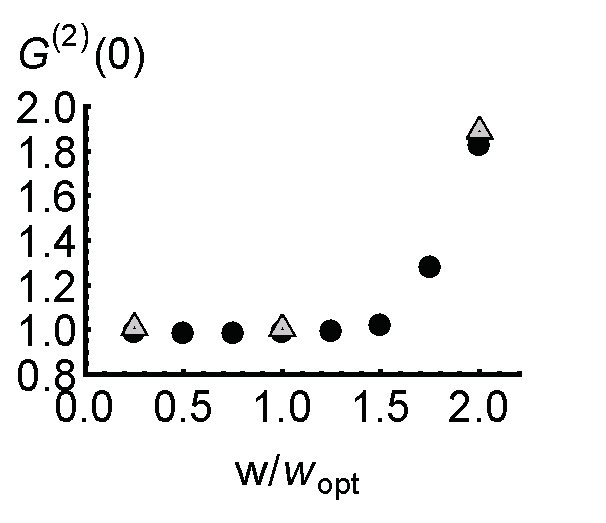
\includegraphics[scale =0.38] {N40LaserG2.eps}\\ \vspace{1mm}
	\hspace{5mm}(a)\hspace{30mm}(b) \hspace{30mm}(c) \hspace{30mm}(d) \hspace{30mm}(e)
\end{center}
		\vspace{-5mm}
\caption{(Color online) Comparison of the different solution methods in
the superradiance ($\xi=0.2$), crossover ($\xi=1$), and lasing ($\xi=5$)
regions for $N=40$ and $C=1$.  The analytic Langevin solution is shown
in red (light gray), the 2nd order cumulant solution is shown in blue
(dark gray), The exact SU4 solution is shown by grey triangles, and the
c-number Langevin simulation results are shown by black circles. The
observables considered are (a) the inversion
$\left<\hat{\sigma}^{z}\right>$, (b) the correlation between atoms
$\left<\hat{\sigma}_{1}^{+} \hat{\sigma}_{2}^{-}\right>$, (c) the
intracavity photon number  $\left<\hat{a}^{\dagger}\hat{a}\right>$, (d)
the linewidth $\Delta \nu$, and (e) the intensity correlation function
$G^{(2)}(0)$.}
\label{N40Comparison}
\end{figure*}

\section{Characterization of the Crossover}
\label{sec:CrossoverCharacterization}

\dmcomment{Need to give more context/motivation here}
A characterization of the parameter space in which a cavity QED system that can be described by Eq.~(\ref{ME1Crossover}) is now given. Since the repumping rate $w$ is varied in a typical experiment, the system is characterized by considering the value $w=w_{opt}$, at which there is a maximum number of intra-cavity photons. We define the crossover parameter $\xi$ to be the ratio of the modified atomic linewidth (including repumping $w$ and dephasing $1/T_2$) evaluated at $w=w_{opt}$, to the cavity linewidth $\kappa$,
\begin{equation}
\xi\equiv\frac{ w_{opt}+\gamma+\frac{1}{T_2}}{4\kappa}.
\label{CrossoverParameter}
\end{equation}
Inserting Eq.~(\ref{wopt}) into  Eq.~(\ref{CrossoverParameter}) yields,
\begin{equation}
\xi\equiv \frac{N \Omega^2}{8\kappa^2}.
\label{CrossoverParameter2}
\end{equation}
Eq.~(\ref{adaopt}) can then be used to rewrite $\xi$ in terms of $(|a_0|^2)_{opt}$ which motivates the use of $\xi$ to characterize the crossover, since then,
\begin{equation}
\xi = \frac{(|a_0|^2)_{opt}}{N},
\end{equation}
i.e. it is proportional to the ratio of the intra-cavity photon number to atom number, or the ratio of the importance of stimulated emission to collective atomic effects.

If $\xi\ll1$, the system is in the bad cavity or superradiant regime. If $\xi\gg1$ our system is in
the good cavity or laser regime. If $\xi\sim1$, the system is in the intermediate regime.

\section{Results}
\label{sec:Results}

\begin{figure*}
\begin{center}
	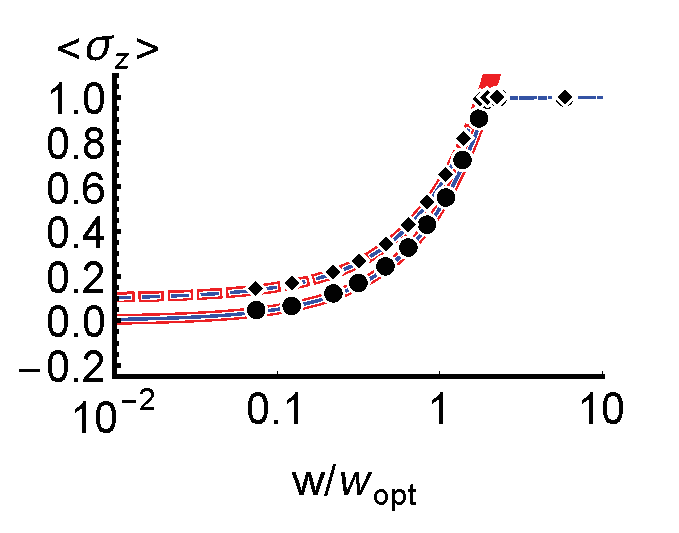
\includegraphics[scale =0.445] {N10000SZ.eps}
	\hspace{-5.0mm} 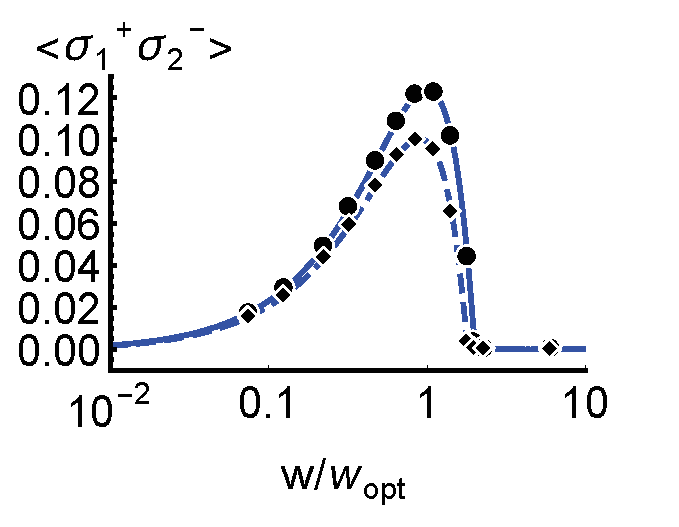
\includegraphics[scale =0.445] {N10000SPSM.eps}
	\hspace{-6.5mm} 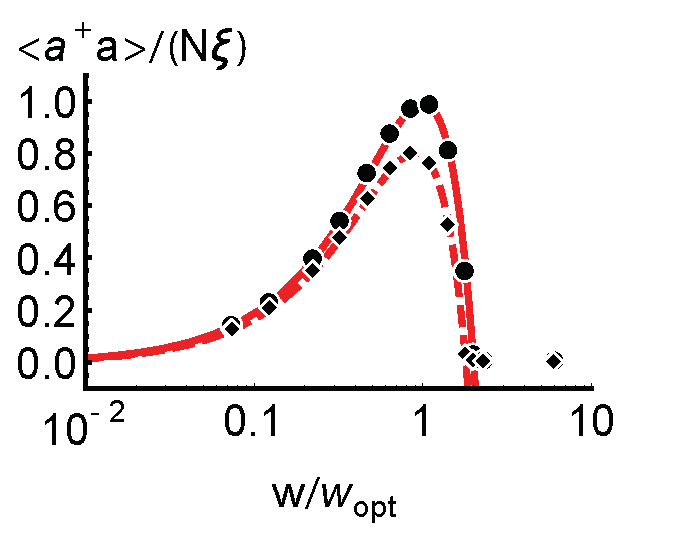
\includegraphics[scale =0.445] {N10000ada.eps}
	\hspace{-5.5mm} 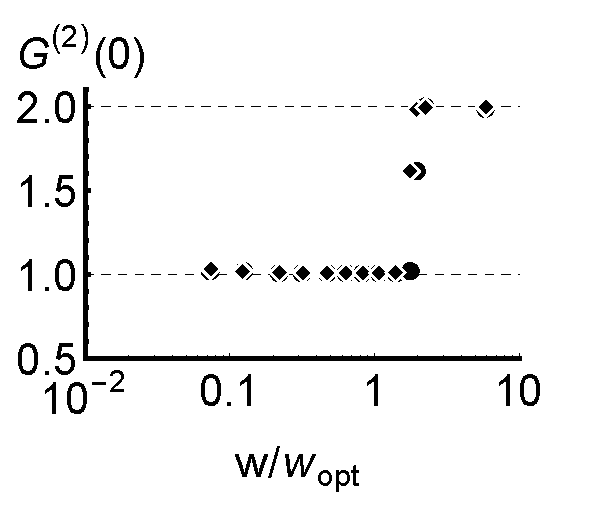
\includegraphics[scale =0.445] {N10000G2S.eps}\\
	\textbf{(a) Universal}\\
	\line(1,0){500}\\
	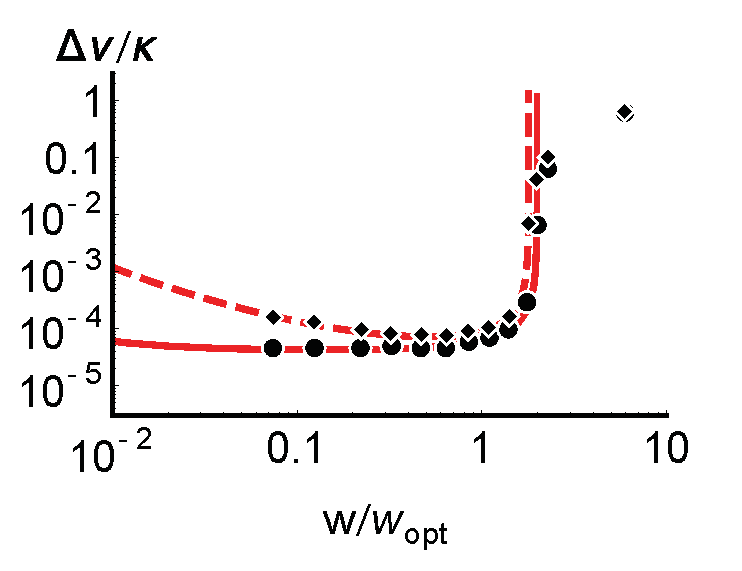
\includegraphics[scale =0.51] {N10000LWS.eps}
	\hspace{-5.5mm} 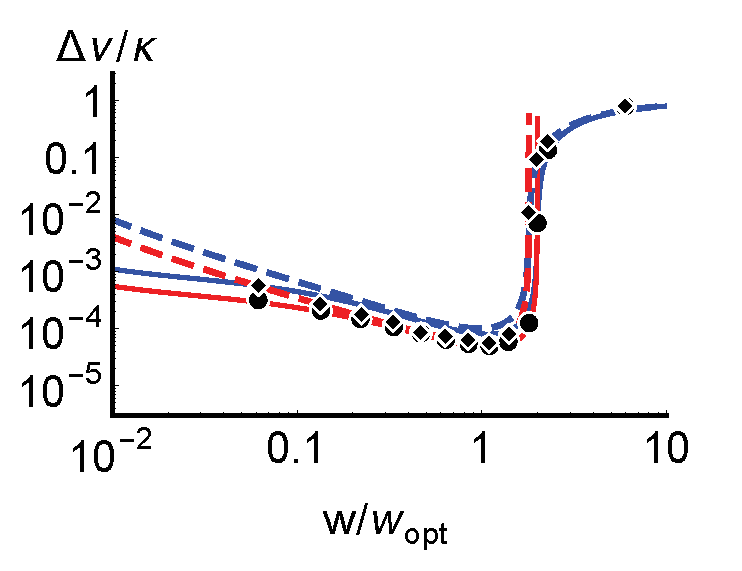
\includegraphics[scale =0.51] {N10000LWC.eps}
	\hspace{-5.5mm} 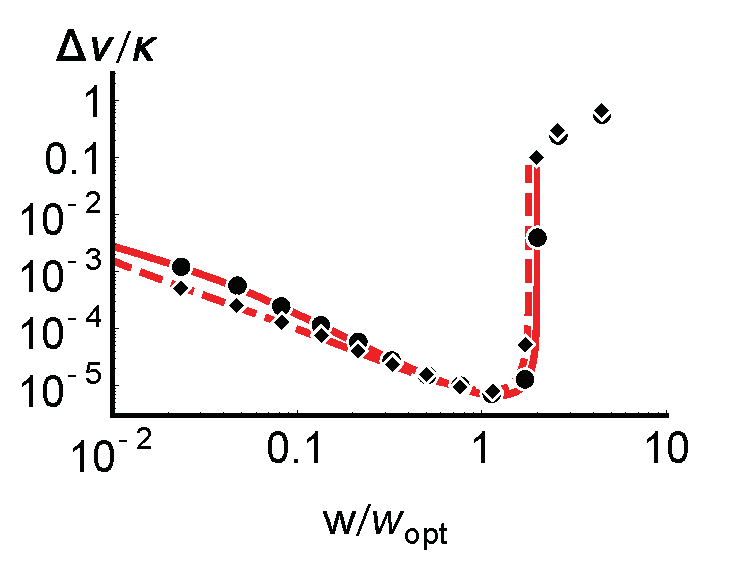
\includegraphics[scale =0.51] {N10000LWL.eps}\\
	\hspace{-10mm}\textbf{(b) Superradiance}\hspace{33mm}\textbf{(c) Crossover}
  \hspace{37mm}\textbf{(d) Lasing}
\end{center}
		\vspace{-5mm}
\caption{(Color online) Solutions using the various methods in the
superradiance ($\xi=0.1$), crossover ($\xi=1$), and lasing ($\xi=10$)
regions for N=10000 and $C=0.1$. For $1/T_2=0$, the analytic Langevin
solution is shown in solid red (solid light gray), the 2nd order
cumulant solution is shown in solid blue (solid dark gray), and the
c-number Langevin simulation results are shown by black circles. For
$1/T_2=\frac{1}{5} w_{opt}$, the analytic Langevin solution is shown in
dashed red (dashed light gray), the 2nd order cumulant solution is shown
in dashed blue (dashed dark gray), and the c-number Langevin simulation
results are shown by black diamonds. (a) All observables considered
except linewidth  $\Delta \nu$ show universal behavior in the
superradiance, crossover, and lasing regions, after appropriate scaling.
The red (light gray) curves have been artificially widened in order to
be seen underneath the blue curves. (b)  $\Delta \nu / \kappa$ in the
superradiance region (c) $\Delta \nu / \kappa$ in the crossover region,
(d) $\Delta \nu / \kappa$ in the lasing region.}
 \label{N10000Comparison}
\end{figure*}


\subsection{Simulations with $N=40$}

As mentioned previously, the SU(4) method is capable of yielding exact
solutions to our model for $N=40$. This is a large enough number of
atoms to expect our three solution methods to be reasonably accurate. We
therefore first compare the analytic Langevin method, the c-number
Langevin method, and the 2nd order cumulant method to the exact SU(4)
result for three different values of the crossover parameter:
$\xi=0.2$, $\xi=1$, and $\xi=5$, which put the system in the
superradiance, crossover, and lasing parameter regions, respectively.
This comparison, seen in Fig.~\ref{N40Comparison}, is made for $N=40$.
The SU(4) method becomes more computationally intensive as $\xi$ is
increased, since there are more photons as $\xi$ is increased, and hence
more basis states need to be tracked. Therefore, for $\xi=5$, the method
that combines the SU(4) with quantum jump method was used. This
simulation was very computationally intensive, so that only a few points
are included.

Fig.~\ref{N40Comparison} shows that there is an excellent agreement
between c-number Langevin and the exact SU(4) theory for $N=40$, in all
parameter regions, for all of the considered observables. Therefore, the
c-number Langevin theory can be relied upon for larger atom numbers,
where it is not possible to apply the SU(4) theory.

The analytic Langevin solution works well in the region around
$w/w_{opt}=1$, but disagrees outside that region. That is because in
Fig.~\ref{N40Comparison} (a) and (c), the analytic Langevin solution
excludes all quantum fluctuations. In Fig.~\ref{N40Comparison} (d),
while the leading order of quantum fluctuations are included, it is
assumed that only phase fluctuations are present, which is not true away
from $w/w_{opt}=1$.

The 2nd order cumulant solution works well qualitatively in all
parameter regions, but as seen in Fig.~\ref{N40Comparison} (b) and (c)
in the superradiance row, and in column (d), there is a quantitative
disagreement between this theory and the SU(4) and c-number Langevin
theories.

This quantitative disagreement is due to the fact that there is a
difference between a Gaussian theory, one in which all moments factorize
into products of no higher than second order moments, and a theory that
uses Gaussian noise. This difference can be seen by considering the
third order moment $\left< \hat{a}^{\dagger}\hat{a}\hat{\sigma}_i^z
\right>$. According to the cumulant theory, $\left<
\hat{a}^{\dagger}\hat{a}\hat{\sigma}_i^z \right>=\left<
\hat{a}^{\dagger}\hat{a}\right> \left<\hat{\sigma}_i^z \right>$, a fact
which was essential to use in deriving the closed the set of equations
used to find the spectrum, Eqns.~(\ref{TwoTimeCE1}). In the Langevin
theory, however, $\left< \hat{a}^{\dagger}\hat{a}\hat{\sigma}_i^z
\right> \neq \left< \hat{a}^{\dagger}\hat{a}\right>
\left<\hat{\sigma}_i^z \right>$, a fact we have checked with our
Langevin simulations. Even though the difference between $\left<
\hat{a}^{\dagger}\hat{a}\hat{\sigma}_i^z \right>$ and $\left<
\hat{a}^{\dagger}\hat{a}\right> \left<\hat{\sigma}_i^z \right>$
decreases as $\frac{1}{N}$, it is precisely the $\frac{1}{N}$ terms that
gives rise to the linewidth according to the cumulant theory.  Therefore
the $25\%$ disagreement between the Langevin and cumulant theories for
large N is not surprising.

The merit of the 2nd order cumulant theory lies in its simplicity. It is
simple to derive the cumulant equations and it is not computationally
intensive to solve them numerically, while the theory still captures the
correct qualitative behavior of the system.


\subsection{Simulations with $N=10000$}

Now that an agreement between the c-number Langevin and exact SU(4)
theories has been established, we study more experimentally realistic
systems with $N=10000$ by applying c-number Langevin theory. We also
include the analytic Langevin and 2nd order cumulant theories for
reference. The results of these simulations can be seen in
Fig.~\ref{N10000Comparison}. Both the situation in which $1/T_2=0$ and
in which $1/T_2=w_{opt}/5$ are considered.

As seen in Fig.~\ref{N10000Comparison} (a), when $1/T_2=0$, the
inversion $\left<\hat{\sigma}^{z}\right>$, the correlation between atoms
$\left<\hat{\sigma}_{1}^{+} \hat{\sigma}_{2}^{-}\right>$, the
intracavity photon number  $\left<\hat{a}^{\dagger}\hat{a}\right>$,  and
the intensity correlation function $G^{(2)}(0)$ all show universal
behavior in the superradiance, crossover, and lasing regimes after
appropriate scaling. When $1/T_2$ is large, $1/T_2=w_{opt}/5$, these
observables still show universal behavior after appropriate scaling, and
do not change their values significantly from the $1/T_2=0$ case.

It is worth noting that even though  $\left<\hat{\sigma}_{1}^{+}
\hat{\sigma}_{2}^{-}\right>$ has universal behavior throughout the
crossover, typical lasers are operated just above threshold at $w \ll
w_{opt}$, where the resulting value of
$\left<\hat{\sigma}_{1}^{+}\hat{\sigma}_{2}^{-}\right>_{opt}$ is much
smaller, which is why atom-atom correlations are not usually thought to
be important in lasers.

The linewidth $\Delta \nu$, however, does not show universal behavior in
the superradiance, crossover, and lasing regimes. As seen in
Fig.~\ref{N10000Comparison} (b), in the superradiance region, when
$1/T_2=0$, $\Delta \nu / \kappa$ is flat in the region of $w/w_{opt}<1$.
In contrast, the linewidth in the lasing regime, shown in
Fig.\ref{N10000Comparison} (d), linearly increases with increasing
$w_{opt}$. This is the typical Schawlow-Townes behavior, which can be
seen by considering $\left<\hat{a}^{\dagger}\hat{a}\right>/\kappa$ using
Eq.~(\ref{a0sqSS}). In the crossover region, shown in
Fig.~\ref{N10000Comparison} (c), we see that for $w/w_{opt}$ small,
$\Delta \nu/\kappa$ is flat, and as $w/w_{opt}$ approaches unity,
$\Delta \nu/\kappa$ starts to linearly decrease as in the lasing regime.
Therefore, a system in the crossover region displays characteristics of
both superradiance and lasing.
\dmcomment{The previous sentence was commented out. Do we want this in
  the paper? Perhaps rephrase a bit?}

\begin{figure}
\begin{center}
	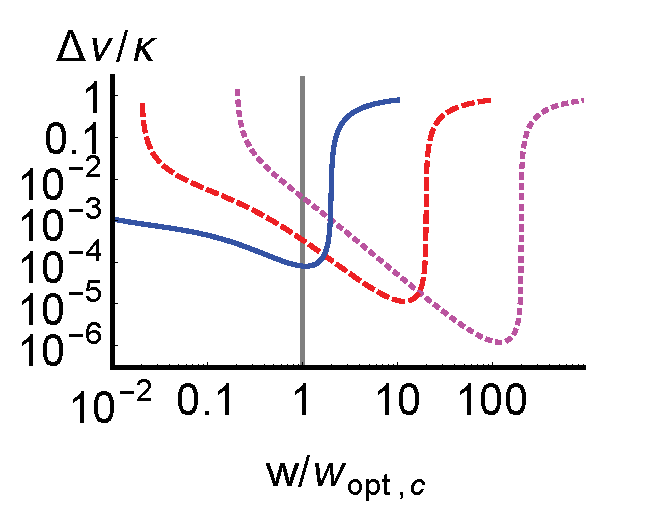
\includegraphics[scale =0.42] {LinewidthComparison.eps}
	\hspace{-4.5mm} 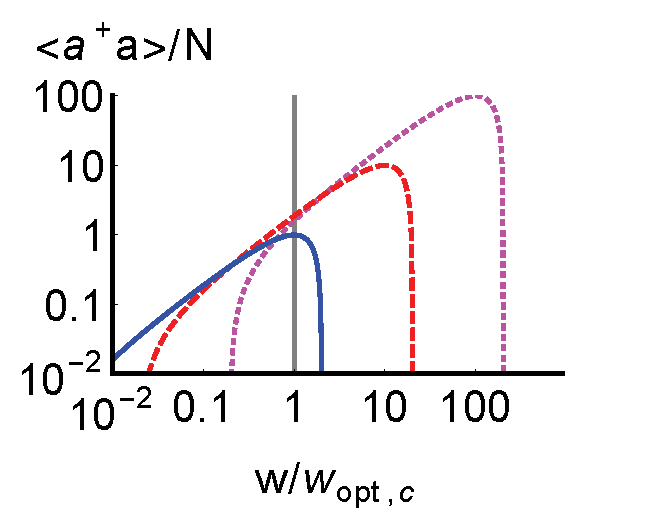
\includegraphics[scale =0.42] {adaComparison.eps}\\
	\hspace{-3mm}\textbf{(a)}\hspace{37mm}\textbf{(b)} \hspace{35mm}
\end{center}
		\vspace{-5mm}
\caption{(Color online) Comparison of (a) linewidth and (b) Intracavity
intensity for a system operated in the crossover ($\xi=1$) shown in blue
solid, lasing ($\xi=10$) shown in red dashed, and far lasing ($\xi=100$)
shown in magenta dotted, regions. $w_{opt,c}$ is the optimum $w$ value
in the crossover region. For all systems, $N=10000$.}
\label{LWadaComparison}
\end{figure}

When $1/T_2$ is increased to $1/T_2=w_{opt}/5$,
Fig.~\ref{N10000Comparison} (b) shows that $\Delta \nu/\kappa$ is
increased for $w/w_{opt}$ small, but it is not significantly affected by
$1/T_2$ as $w/w_{opt}$ approaches unity. In any case, this is the region
in which a superradiant system should be operated, since this is the
region of maximum intracavity intensity.

In the crossover region, seen in Fig.~\ref{N10000Comparison} (c), when
$1/T_2=w_{opt}/5$, $\Delta \nu/\kappa$ is increased for $w/w_{opt}$
small, where the system is displaying superradiant behavior, but is
completely insensitive to $w/w_{opt}$ approaching unity, where the
system starts to display lasing behavior.

As seen in Fig.~\ref{N10000Comparison} (d), in the lasing region, when
$1/T_2=w_{opt}/5$, $\Delta \nu/\kappa$ is not increased, but actually
decreased in the region slightly below $w/w_{opt}=1$, when compared to
the $1/T_2=0$ case. This reduction has also been observed for smaller
atom numbers using the exact SU(4) code. It can be shown that the value
of $1/T_2$ that maximally reduces the linewidth is
$1/T_2=\frac{w_{opt}}{1+\sqrt{2}}$.

A typical laser is operated just above threshold, where $w/w_{opt} \ll
1$. As seen in Fig.~\ref{LWadaComparison} (a), for the same pump
strength $w$, and a fixed $N$, a system in the crossover region could be
operated with $w/w_{opt} = 1$, allowing the crossover system to have a
linewidth orders of magnitude smaller than the linewidth of the lasing
system. Fig.~\ref{LWadaComparison} (b) shows that the intracavity
intensity, $\left<\hat{a}^{\dagger}\hat{a}\right>$, will be roughly the
same for the crossover system operated at $w/w_{opt} = 1$ as for a laser
system operated at  $w/w_{opt} \ll 1$.


\subsection{Effect of Cavity and Atomic Level Instabilities on the
Spectrum}

The effect of instabilities in the cavity frequency and atomic frequency
on the linewidth is now investigated. Cavity frequency instability can
be caused by fluctuations in cavity length due to the thermal
fluctuations of the cavity mirrors, which are unavoidable in an
experiment. The energy levels in an atom can also be shifted by stray
electromagnetic fields. The frequency of the combined atom-cavity system
$\omega$ lies somewhere between the bare atom and cavity frequencies,
and is given by Eq.~(\ref{atomcavityfrequencycenter1}).

If $\omega$ is varied, the resultant time averaged linewidth will be an
average over these values, and will hence be much broader than the
quantum limited linewidth. Therefore, the derivative of  $\omega$ with
respect to $\omega_c$, and with respect to $\omega_a$, gives us an idea
as to how much of an effect an instability in these frequencies will
have on broadening the linewidth. These derivatives are plotted in
Fig.~\ref{CavityInstability}.

\begin{figure}
\begin{center}
	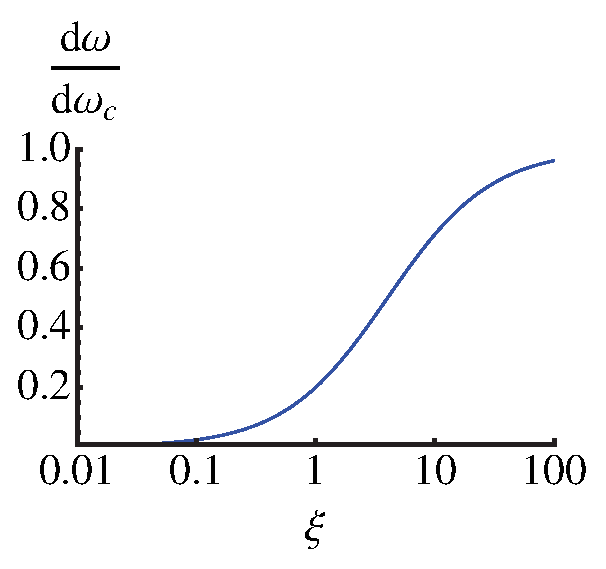
\includegraphics[scale=0.44] {CavityInstability.eps}
	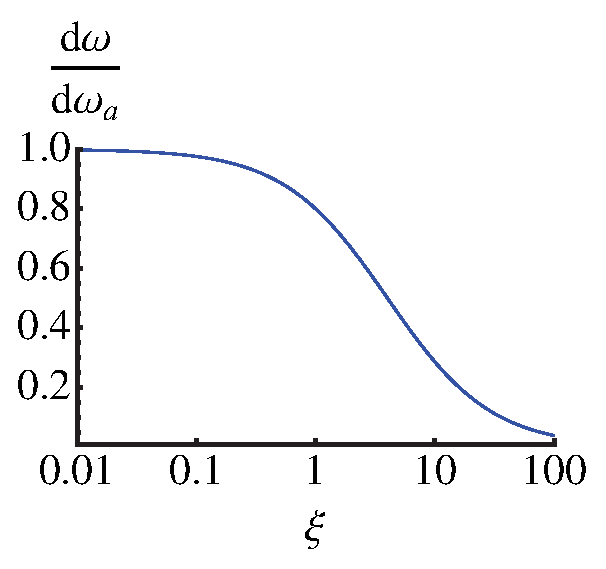
\includegraphics[scale=0.44] {AtomInstability.eps}\\
\hspace{2mm} \textbf{(a)}\hspace{39mm}\textbf{(b)} \hspace{35mm}
\end{center}
\caption{(Color online) Instability in the atom-cavity system frequency
$\omega$ with respect to (a) the cavity frequency $\omega_c$ and (b)
atomic frequency $\omega_a$ as a function of crossover parameter $\xi$}
\label{CavityInstability}
\end{figure}
Fig.~\ref{CavityInstability} (a) tells us that on the lasing side of the
crossover, $\omega$ is shifted proportionally to the shift in
$\omega_c$, while on the superradiant side, $\omega$ is insensitive to
shifts in $\omega_c$.  Conversely, in Fig.~\ref{CavityInstability} (b)
it can be seen $\omega$ is shifted proportionally to the shift in
$\omega_a$ on the superradiance side of the crossover, while on the
lasing side, $\omega$ is insensitive to shifts in $\omega_a$. In the
intermediate regime ($\xi=1$), $\omega$ is not as sensitive to a shift
in the $\omega_c$ as it is in the laser regime, and it is not as
sensitive to a shift in the $\omega_a$, as it is on the superradiance
side.


\section{Conclusion}

A model that is capable of describing a system operating in any
parameter region of the crossover between steady state superradiance and
lasing has been introduced, and four solution methods to that model were
demonstrated. The first method combines the SU(4) and quantum jump
methods, and is capable of describing systems with more photons than
just the SU(4) method alone.  We also introduced a method that solves a
set of c-number Langevin equations that approximate the quantum Langevin
equations that are equivalent to our model. This method was seen to have
outstanding agreement with the exact SU(4) method. Analytic expressions
for the expectation values of the quantum Langevin equations were then
derived. Along with these solutions, an analytic solution for the
linewidth of the power spectrum, which assumes Gaussian phase
fluctuations, and neglects amplitude fluctuations was derived. It is
demonstrated that these analytical results agree with SU(4) and c-number
Langevin methods in the region in which the value of re-pumping is such
that the system has the maximum number of intra-cavity photons, but
disagree far from this region. Finally, a closed set of equations to
second order in a cumulant expansion were derived, and shown to agree
qualitatively with the SU(4) and c-number Langevin methods.

Although a system in the lasing parameter region is capable of
possessing the smallest linewidth, typically lasers operate with a
re-pumping rate that puts them just above threshold, which does not
allow the smallest linewidth for the system to be realized. For the same
re-pumping rate, a system operating in the crossover region will be much
farther above threshold, potentially allowing for a linewidth orders of
magnitude smaller than in the laser region. Also, a crossover system
will have a larger intracavity intensity than a superradiant system,
making the former more experimentally accessible.

It was also demonstrated that a system in all regions of the crossover
is insensitive to atomic dephasing as long as the re-pumping rate is
smaller than the dephasing rate. Also, as the crossover is traversed
into the lasing region, atomic dephasing can actually cause a reduction
in the linewidth.

Finally, it was shown that the linewidth on the superradiance side is
insensitive to fluctuations in cavity length, and that these
fluctuations become more important as the crossover is traversed toward
the laser side. Conversely, it was shown that the linewidth on the
lasing side is insensitive to fluctuations in the atomic energy levels,
and that these fluctuations become more important on the superradiance
side. A system in the crossover region will be less sensitive to cavity
frequency fluctuations than a lasing system, and it will be less
sensitive to atomic frequency instabilities than a superradiant system.
Both of these fluctuations cause a broadening of the linewidth. These
conclusions are significant since fluctuations in the cavity frequency
are a principal limitation preventing further reduction of the linewidth
in today's most ultrastable lasers.

This work has been supported by JILA-NSF-PFC-1125844, DARPA, QuASAR, and
NIST.


\bibliographystyle{unsrt}
\bibliography{CrossoverPaper}

\end{document}

